

\subsection{开发语言}
Kubernetes生态的主流语言是Go,
在Serverless平台的开发中,
关于开发语言的资料相对较少,
但根据现有资料,
可以了解和推测:

\begin{itemize}
    \item 基于Kubernetes、Knative等Kubernetes生态的系统以Go为主;
    包括EasyFaaS、firecracker-containerd等也是使用Go开发
    \item 美团在建设Nest平台时没有选择Go而选择了Java作为主要语言,
    原因是因为美团内部Java占主导地位\cite{meituan_serverless_nest};
    另外Apache OpenWhisk主要是Scala实现
    \item Rust有较多的应用,例如Firecracker使用Rust开发,字节使用了Rust/WebAssembly\cite{bytedance_faas}
\end{itemize}

\subsection{架构设计}
典型的Serverless架构是基于事件驱动的模式,
根据调用模型又可以分为同步模式和异步模式两种,
因此我们可以按照功能把整体Serverless的架构分为如下几个部分:

\begin{itemize}
    \item 事件路由:作为Serverless的调用入口,负责响应用户请求
    \item 工作负载:负责最终执行负载(函数或者自定义镜像)
    \item 辅助服务:除此之外的其他组件都可以归并为辅助工作负载执行或者事件触发的范畴之中,
    例如管理工作负载的生命周期、镜像拉取等各种功能
\end{itemize}

\subsubsection{AWS Lambda的架构}
AWS Lambda在Serverless领域耕耘最久、积累最丰富,
因此Lambda的架构十分具有参考价值。
AWS Lambda从发布之初到现在也经历过许多变化,
包含新功能的支持、架构的调整等,
如\cref{lambda_involution}所示。

\begin{figure}[ht!]
    \centering
    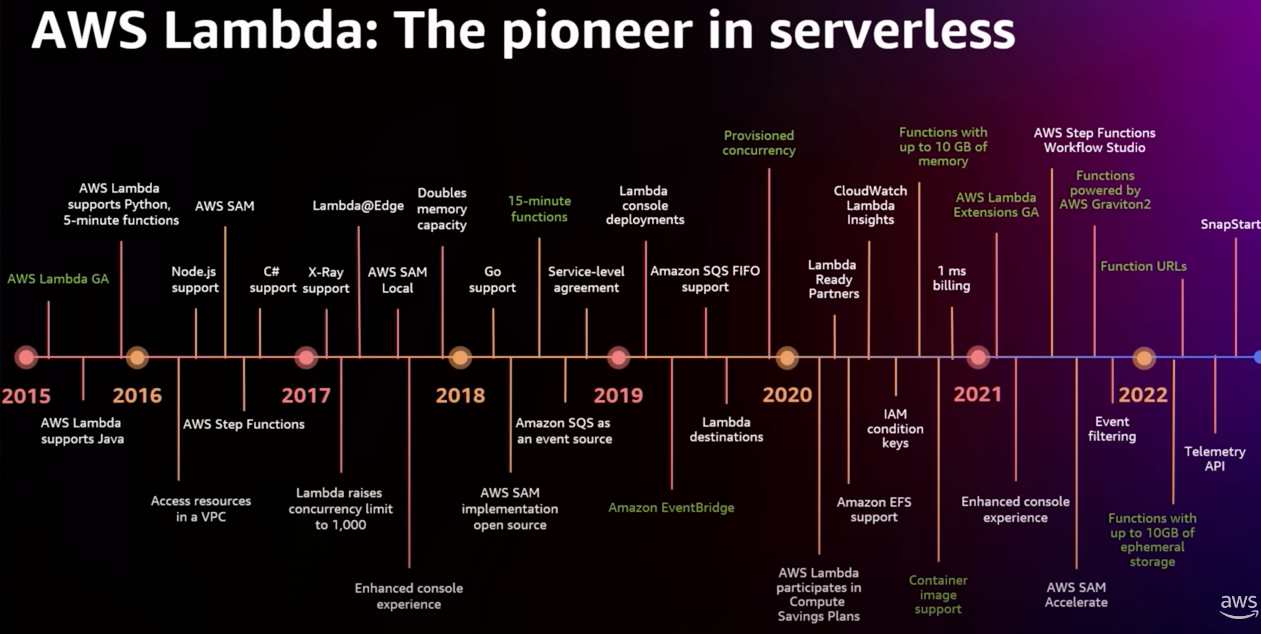
\includegraphics[width=\linewidth]{images/lambda_involution.png}
    \caption{AWS Lambda演进历史\cite{aws_lambda_2022}}
    \label{lambda_involution}
\end{figure}



\subsection{高可用保障}

\subsubsection{异地多分区}
高可用主要需要解决的问题是容忍分布式故障,
基于Kubernetes的架构自身有一定的容忍能力,
但单个Kubernetes集群存在伸缩瓶颈\cite{k8s_large_cluster},
且隔离程度有限,
因此通常采取多集群的方式实现异地容灾、业务隔离和高可用,
例如美团、字节均采取这种方式\cite{meituan_serverless_nest, bytedance_faas}。
美团的异地多集群架构如\cref{nest_arch}所示。

\begin{figure}[ht!]
    \centering
    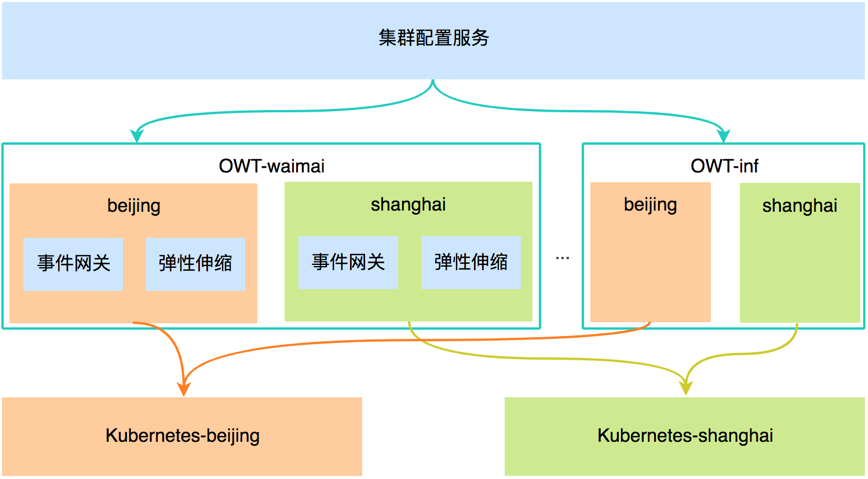
\includegraphics[width=0.7\linewidth]{images/nest_k8s_arch.png}
    \caption{美团Nest的部署架构}
    \label{nest_arch}
\end{figure}

对于规模更大的公有云例如AWS,
采取的是分地域+可用区的方式,
一方面实现隔离和高可用,
另一方面可以就近服务而提升性能\cite{aws_global_infra}。

\subsubsection{并发度限制}
尽管理论上Serverless具有无限的扩容能力,
但主流的Serverless平台都会进行并发限制,
通常有设置并发度的选项。
AWS默认每个区域为1000QPS
\footnote{AWS的并发限制是可以申请增加的,不设定上限,但需要提前申请。}\cite{lambda_concurrency};
Google Cloud Run单个容器默认限制为80,最高可设置为1000\cite{google_cloud_run_concurrency};
美团在事件网关上进行限流,
并支持对后端函数进行降级和限流\cite{meituan_serverless_nest}。

\subsection{隔离及安全}
\subsubsection{隔离策略}
FaaS系统中,资源隔离是必须的。
从资源利用的角度来说,需要隔离不同的函数运行实例,
使其相互之间不受影响,例如AWS运行Lambda最小的实例内存为128Mb,
而典型的宿主机实例则大至384Gb内存。
另一方面,从安全的角度来说,
用户代码是不可信代码,
如何防止攻击、保证底层系统安全,
也需要对函数运行进行隔离。

常规的Docker实现依赖Linux内核提供的groups、namespaces等机制实现隔离,
AWS基于Firecracker/microVM实现了自己的多层安全策略,
在性能/安全之间进行了较好的平衡,
如\cref{firecracker_isolation_model}所示\cite{Agache2020, aws_2020_function_isolation}。
这种模式的一个附加的好处是,
可以更灵活地进行监控。

\begin{figure}[ht!]
    \centering
    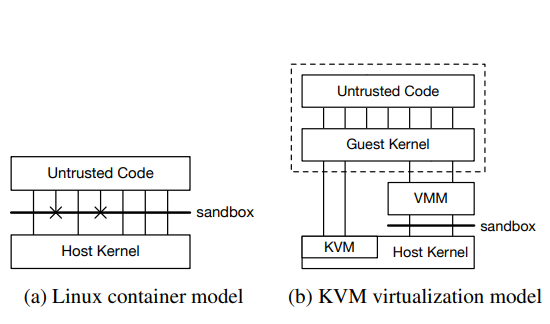
\includegraphics[width=0.7\linewidth]{images/firecrack-isolation.png}
    \caption{Docker与Firecracker的隔离方式对比\cite{Agache2020}}
    \label{firecracker_isolation_model}
\end{figure}

一些Serverless平台即支持FaaS,
也支持CaaS,
这两种模式的最终运行方式有所区别,
因此有将这两种模式的运行时进行隔离的做法,
例如字节的FaaS平台架构就采取了不同的K8s集群运行函数负载和镜像负载,
如\cref{bytedance_faas_arch}所示。

\begin{figure}[ht!]
    \centering
    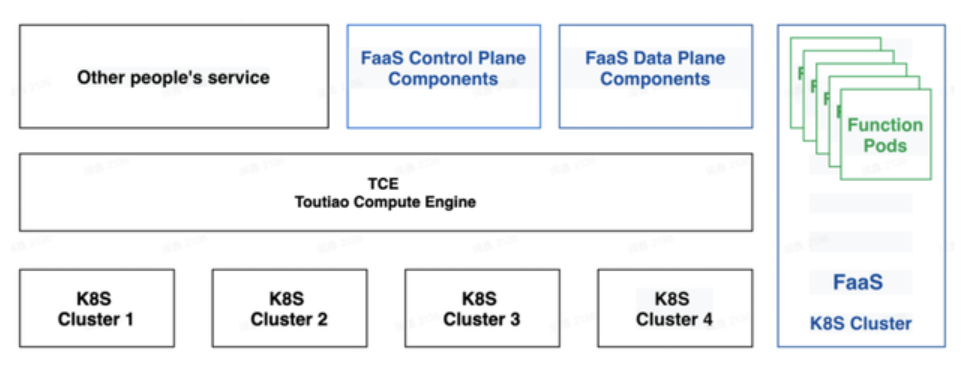
\includegraphics[width=0.7\linewidth]{images/bytedance_faas_arch.png}
    \caption{字节跳动FaaS平台架构\cite{bytedance_faas}}
    \label{bytedance_faas_arch}
\end{figure}

\subsubsection{安全容器}
由于容器技术是操作系统级的虚拟化技术,
它的安全性比虚拟机要差,
因此有一些技术用来增强容器的安全性,
也称之为安全容器技术,
例如Kata Container和Firecracker
\footnote{严格意义上Firecracker是一种轻量级虚拟技术(MicroVM)。},
以及在Kata基础上优化的RunD\cite{rund}。

\subsection{冷启动}